% example.tex
%
% Copyright (C) 2010,2011 Laura Dietz
% Copyright (C) 2012 Jaakko Luttinen
%
% This file may be distributed and/or modified
%
% 1. under the LaTeX Project Public License and/or
% 2. under the GNU General Public License.
%
% See the files LICENSE_LPPL and LICENSE_GPL for more details.

\documentclass[a4paper]{article}

\usepackage{tikz}
\usepackage{amsmath}
\usetikzlibrary{bayesnet}
\usepackage{apacite}
%\pgfrealjobname{example} % name of this file

\title{Supplementary material to real-time lexical comprehension in young children learning American Sign Language}
\author{Kyle MacDonald, Todd LaMarr, Virginia A. Marchman,\\ David Corina, and Anne Fernald}
\date{}

\begin{document}

\maketitle

In this document, we present two pieces of supplemental information. First, we provide details about the Bayesian models used to analyze our data. Second, we show a sensitivity analysis that provides evidence that our estimates of the associations between age/vocabulary and accuracy/reaction time (RT) are robust to different parameterizations of the prior distribution and different cutoffs for the analysis window. 

\section{Model specifications}

Our key analyses use Bayesian linear models to test our hypotheses of interest and to estimate the associations between age/vocabulary and RT/accuracy. Figure 1 (Accuracy) and 2 (RT) present graphical models that represent all of the data, parameters, and other variables of interest, and their dependencies. Latent parameters are shown as unshaded nodes while observed parameters and data are shown as shaded nodes. All models were fit using JAGS software \cite{plummer2003jags} and adapted from models in \citeA{kruschke2014doing} and \citeA{lee2014bayesian}.

\subsection{Accuracy}

To test the association between age/vocabulary and accuracy. We assume each participant's mean accuracy is drawn from a Gaussian distribution with a mean, $\mu_i$, and a standard deviation, $\sigma$. The mean is a linear function of the intercept, $\alpha$, which encodes the expected value of the outcome variable when the predictor is zero, and the slope, $\beta$, which encodes the expected change in the outcome with each unit change in the predictor (i.e., the strength of association). 

For $\alpha$ and $\sigma$, we use vague priors on a standardized scale, allowing the model to consider a wide range of plausible values. Since the slope parameter $\beta$ is critical to our hypothesis of a linear association, we chose to use an informed prior: that is, a truncated Gaussian distribution with a mean of zero and a standard deviation of one on a standardized scale. Centering the distribution at zero is conservative and places the highest prior probability on a null association, to reduce the chance that  our model overfits the data. Truncating the prior encodes our directional hypothesis that accuracy should increase with age and larger vocabulary size. And using a standard deviation of one constrains the plausible slope values, thus making our alternative hypothesis more precise. We constrained the slope values based on previous research with children learning spoken language showing that the average gain in accuracy for one month of development between 18-24 months to be $\sim$0.016 \cite{fernald2008looking}.

\begin{figure}[ht]
  \begin{center}
    % model_lda.tex
%
% Copyright (C) 2010,2011 Laura Dietz
% Copyright (C) 2012 Jaakko Luttinen
%
% This file may be distributed and/or modified
%
% 1. under the LaTeX Project Public License and/or
% 2. under the GNU General Public License.
%
% See the files LICENSE_LPPL and LICENSE_GPL for more details.

% Latent Diriclet allocation model

%\beginpgfgraphicnamed{model-lda}

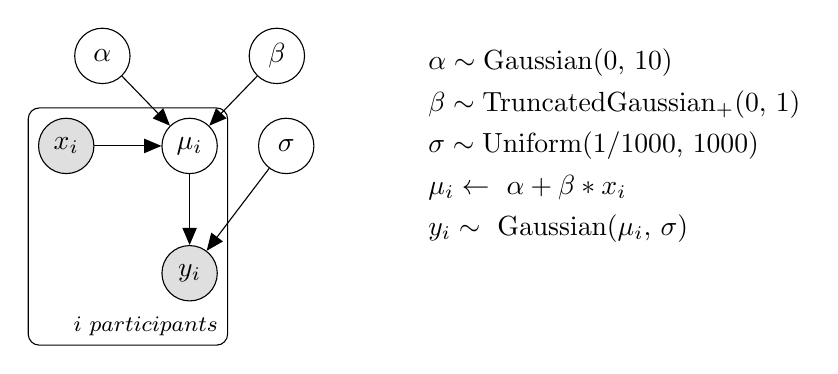
\begin{tikzpicture}[x=1.7cm,y=1.8cm]

 % Nodes

\node[obs] (y) {$y_i$}; 
\node[latent, above=	0.5 of y]   (mu)   {$\mu_i$};
\node[latent, right=	0.3 of mu]   (sigma)   {$\sigma$};
\node[obs, left=0.5 of mu]   (x)   {$x_i$};


\node[latent, above left =0.5 of mu]   (alpha)   {$\alpha$};
\node[latent, above right=0.5 of mu]   (beta)   {$\beta$};

\node[right=1.5 of mu] {
 $\begin{aligned}
     &\alpha \sim \text{Gaussian(0, $10$)}\\
     &\beta \sim \text{TruncatedGaussian$_+$(0, 1)}\\
     &\sigma \sim \text{Uniform($1/1000$, 1000)}\\
     &\mu_i \leftarrow\ \alpha + \beta \ast x_i\\ 
     &y_i \sim\ \text{Gaussian($\mu_i$, $\sigma$)}
  \end{aligned}$
};


% Connect nodes
  \edge[->] {mu, sigma} {y};
  \edge[->] {x, alpha, beta} {mu} ;
 
   % Plates
  \plate {} {
        (x)(y)
  } {$i\ participants$};

\end{tikzpicture}
%\endpgfgraphicnamed

%%% Local Variables: 
%%% mode: tex-pdf
%%% TeX-master: "example"
%%% End: 

  \end{center}
  \caption{Graphical model representation of the linear regression used to predict accuracy. The shaded nodes represent observed data (i.e., the $i$th participant's age, vocabulary, and mean accuracy). Unshaded nodes represent latent parameters (i.e., the intercept and slope of the linear model).}
\end{figure}

\begin{figure}[ht]
  \begin{center}
    % model_lda.tex
%
% Copyright (C) 2010,2011 Laura Dietz
% Copyright (C) 2012 Jaakko Luttinen
%
% This file may be distributed and/or modified
%
% 1. under the LaTeX Project Public License and/or
% 2. under the GNU General Public License.
%
% See the files LICENSE_LPPL and LICENSE_GPL for more details.

% Latent Diriclet allocation model

%\beginpgfgraphicnamed{model-lda}

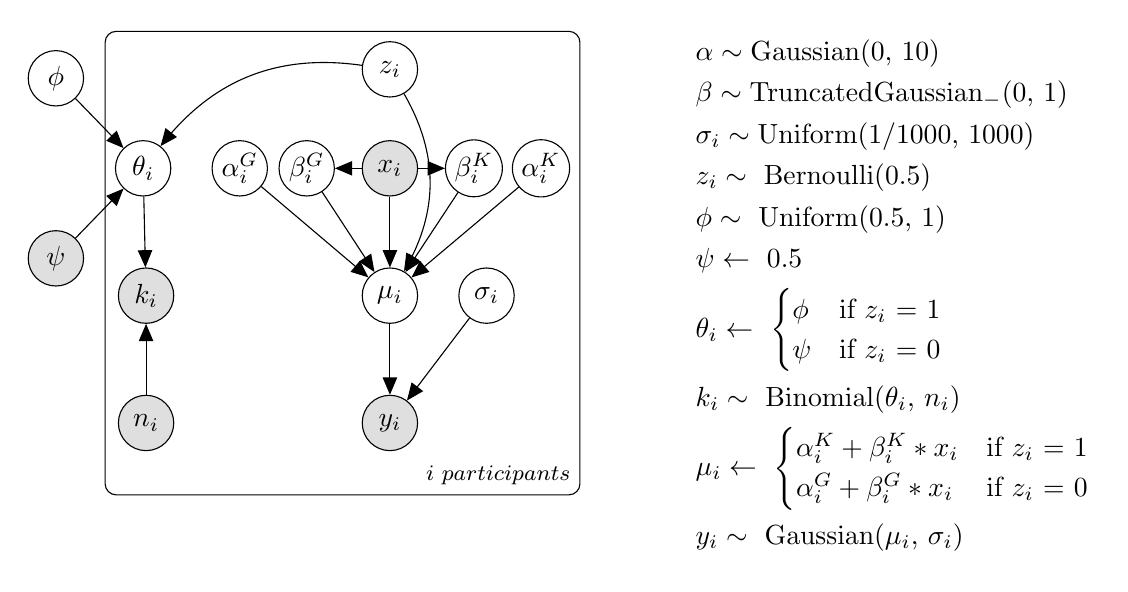
\begin{tikzpicture}[x=1.7cm,y=1.8cm]

% Box around BLR
% \draw[red, line width=0.5mm, dashed,] (-1.5,-0.25) -- (1.5,-0.25) -- (1.5, 2.25) -- (-1.5, 2.25) -- cycle;
 % Nodes
\node[obs] (y) {$y_i$}; 
\node[latent, above=	0.5 of y]   (mu)   {$\mu_i$};
\node[latent, right=	0.3 of mu]   (sigma)   {$\sigma_i$};
\node[obs, above=0.5 of mu]   (x)   {$x_i$};
\node[latent, above=	0.3 of x]   (z)   {$z_i$};


\node[latent, left=0.7 of x]   (alpha_g)   {$\alpha_i^G$};
\node[latent, left=0.2 of x]   (beta_g)   {$\beta_i^G$};
\node[latent, right=0.7 of x]   (alpha_k)   {$\alpha_i^K$};
\node[latent, right=0.2 of x]   (beta_k)   {$\beta_i^K$};


\node[latent, left=0.3 of alpha_g]   (theta)   {$\theta_i$};
\node[obs, left=1.4 of y]   (n)   {$n_i$};
\node[obs, above=0.5 of n]   (k)   {$k_i$};
\node[latent, above left=0.5 of theta]   (phi)   {$\phi$};
\node[obs, below left=0.5 of theta]   (psi)   {$\psi$};

\node[right=2 of mu] {
 $\begin{aligned}
     &\alpha \sim \text{Gaussian(0, $10$)}\\
     &\beta \sim \text{TruncatedGaussian$_-$(0, 1)}\\
     &\sigma_i \sim \text{Uniform($1/1000$, 1000)}\\
     &z_i \sim\ \text{Bernoulli(0.5)}\\
     &\phi \sim\ \text{Uniform(0.5, 1)}\\
     &\psi \leftarrow\ \text{0.5}\\
     &\theta_i \leftarrow\ 
        	\begin{cases}
    		\phi & \text{if } z_i \text{ = 1}\\
    		\psi & \text{if } z_i \text{ = 0}\\
 	 \end{cases}\\
     &k_i \sim\ \text{Binomial($\theta_i$, $n_i$)}\\
     &\mu_i \leftarrow\ 
        	\begin{cases}
    		\alpha_i^K + \beta_i^K \ast x_i & \text{if } z_i \text{ = 1}\\
    		\alpha_i^G + \beta_i^G \ast x_i & \text{if } z_i \text{ = 0}\\
 	 \end{cases}\\
     &y_i \sim\ \text{Gaussian($\mu_i$, $\sigma_i$)}
  \end{aligned}$
};


% Connect nodes
  \edge[->] {mu, sigma} {y};
  \edge[->] {x, alpha_g, beta_g, alpha_k, beta_k} {mu} ;
  \path (z) edge [bend left, ->] (mu);
   \path (z) edge [bend right, ->] (theta);
  \edge[->] {x} {beta_g} ;
  \edge[->] {x} {beta_k} ;
   \edge[->] {theta, n} {k} ;
      \edge[->] {phi, psi} {theta} ;
 
   % Plates
  \plate {} {
        (x)(mu)(y)(alpha_g)(alpha_k)(z)(theta)
  } {$i\ participants$};

\end{tikzpicture}
%\endpgfgraphicnamed

%%% Local Variables: 
%%% mode: tex-pdf
%%% TeX-master: "example"
%%% End: 

  \end{center}
  \caption{Graphical model representation of the linear regression plus latent mixture model (i.e., guessing model). The guessing model assumes that each individual participant's first shift is either the result of guessing or knowledge. And the latent indicator $z_i$ determines whether the $i$th participant is included in the linear regression estimating the association between age/vocabulary and RT.} 
\end{figure}

% SOL BDA RT
\subsection{Reaction Time}

The use of RT as a processing measure is based on the assumption that the timing of a child's first shift reflects the speed of their lexical access. Yet, some children have a first shift that seems to be unassociated with lexical access: their first shift behavior appears random. We quantify this possibility for each participant explicitly (i.e., the probability that the participant is a "guesser") and we create an analysis model where participants who were more likely to be guessers have less of an influence on the estimated relations between RT and age/vocabulary 

%\begin{figure}[ht!]
%	{\centering \includegraphics[width=12cm]{supp_prior_dist_plots.png}}
%	\caption{The prior distribution for the slope parameter, $\beta$, for the Accuracy and Reaction Time models. Each panel shows the range of slopes that the model would consider plausible at that parameterization of the standard deviation for the prior. The vertical blue line indicates the slope value based on prior research with children learning spoken language \protect\cite{fernald2008looking}.}\label{fig:coef_plot}
%\end{figure}

To quantify each participant's probability of guessing, we computed the proportion of signer-to-target (correct) and signer-to-distracter (incorrect) shifts for each child. We then used a latent mixture model in which we assumed that the observed data, $k_i$, were generated by two processes (guessing and knowledge) that had different overall probabilities of success, with the "guessing group"having a probability of 50\%, $\psi$, and the "knowledge" group having a probability greater than 50\%, $\phi$. The group membership of each participant is a latent indicator variable, $z_i$, inferred based on that participant's proportion of correct signer-to-target shifts relative to the overall proportion of correct shifts across all participants (see \citeA{lee2014bayesian} for a detailed discussion of this modeling approach). We then used each participant's inferred group membership to determine whether they were included in the linear regression. In sum, the model allows participants to contribute to estimated associations between age/vocabulary and RT \textit{proportional} to our belief that they were guessing. 

As in the Accuracy model, we use vague priors for $\alpha$ and $\sigma$ on a standardized scale. We again use an informed prior for $\beta$, making our alternative hypothesis more precise. That is, we constrained the plausible slope values based on previous research with children learning spoken language showing that the average gain in RT for one month of development between 18-24 months to be $\sim$40ms \cite{fernald2008looking}. 

% SOL SENSITIVITY ANALYSIS
\subsection{Sensitivity Analysis: Priors and Window Selection}

We conducted a sensitivity analysis to show that our parameter estimates for the associations between accuracy/RT and age/vocabulary are robust to decisions about (a) the analysis window and (b) the specification of the prior distribution on the slope parameter. Specifically, we varied the parameterization of the standard deviation on the slope, allowing the model to consider a wider or narrower range of values to be plausible a priori. We also fit these different models to two additional analysis windows +/- 300 ms from the final analysis window: 600-2500 ms (the middle 90\% of the RT distribution in our experiment).

Figure 2 shows the results of the sensitivity analysis, plotting the coefficient for the $\beta$ parameter in each model for the three different analysis windows for each specification of the prior. All models show similar coefficient values, suggesting that inferences about the parameters are not sensitive to the exact form of the priors. Table 1 shows the Bayes Factors for all models across three analysis windows and fit using four different vales for the slope prior. The Bayes Factor only drops below 3  when the prior distribution is quite broad (standard deviation of 3.2) and only for the longest analysis window (600-2800 ms). In sum, the strength of evidence for a linear association is robust to the choice of analysis window and prior specification.

\begin{figure}[hb]
	{\centering \includegraphics[width=12cm]{supp_coef_plot.png}}
	\caption{Coefficient plot for the slope parameter, $\beta$, for four different parameterizations of the prior and for three different analysis windows. Each panel shows a different model. Each point represents a $\beta$ coefficient measuring the strength of association between the two variables. Error bars are 95\% HDIs around the coefficient. Color represents the three different analysis windows. }\label{fig:coef_plot}
\end{figure}

% latex table generated in R 3.2.4 by xtable 1.8-2 package
% Wed May 18 23:51:29 2016
\begin{table}[b]
\centering
\begin{tabular}{lc|rrrr}
  \hline
Window & SD\_Slope & Acc\_Age & Acc\_Vocab & RT\_Age & RT\_Vocab \\ 
  \hline
600\_2200 & 3.2 & 6.2 & 3.7 & 2.4 & 4.1 \\ 
  600\_2200 & 1.4 & 14.1 & 5.5 & 3.5 & 8.6 \\ 
  600\_2200 & 1.0 & 19.4 & 8.9 & 5.0 & 9.2 \\ 
  600\_2200 & 0.7 & 22.7 & 11.6 & 7.8 & 17.0 \\ 
  600\_2500 & 3.2 & 11.0 & 2.3 & 5.6 & 6.1 \\ 
  600\_2500 & 1.4 & 9.7 & 4.0 & 13.8 & 10.5 \\ 
  600\_2500 & 1.0 & 12.8 & 6.8 & 12.5 & 18.2 \\ 
  600\_2500 & 0.7 & 15.6 & 6.8 & 17.9 & 20.7 \\ 
  600\_2800 & 3.2 & 6.0 & 1.1 & 1.2 & 1.4 \\ 
  600\_2800 & 1.4 & 10.7 & 2.6 & 3.5 & 4.7 \\ 
  600\_2800 & 1.0 & 13.5 & 4.0 & 3.7 & 4.0 \\ 
  600\_2800 & 0.7 & 15.2 & 4.6 & 5.5 & 5.6 \\ 
   \hline
\end{tabular}
\caption{Bayes Factors for all four linear models fit to three different analysis windows using four different parameterizations of the prior distribution for the slope parameter $\beta$.} 
\end{table}


\bibliographystyle{apacite}
\clearpage
\bibliography{bda}

\end{document}

%%% Local Variables: 
%%% mode: tex-pdf
%%% TeX-master: t
%%% End: 
